\documentclass[11pt]{beamer}
\usetheme{Warsaw}
\usepackage[utf8]{inputenc}
\usepackage[french]{babel}
\usepackage[T1]{fontenc}
\usepackage{amsmath}
\usepackage{amsfonts}
\usepackage{amssymb}
\usepackage{graphicx}
\usepackage{multicol}
\author{Jean-Dominique FAVREAU \& Arnaud TANGUY}
\title{Détection de composantes principales}
%\setbeamercovered{transparent} 
%\setbeamertemplate{navigation symbols}{} 
%\logo{} 
%\institute{} 
%\date{} 
%\subject{} 
\begin{document}

\begin{frame}
\titlepage
\end{frame}

%\begin{frame}
%\tableofcontents
%\end{frame}
\section{Sphère de Gauss}
\begin{frame}{projection stéréographique}
\begin{multicols}{2}
\begin{figure}[hbtp]
\centering
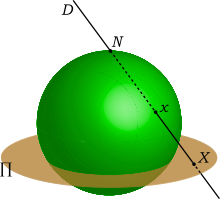
\includegraphics[scale=.6]{220px-Stereo.png}
\caption{Projection stéréographique de la sphère}
\end{figure}
\columnbreak
Soit : \begin{itemize}
\item $N=\left(\begin{array}{l}0\\ 0\\ \alpha\end{array}\right)$
\item $\Pi : z=-\beta$
\item $x=\left(\begin{array}{l}x_1\\ x_2\\ x_3\end{array}\right)$
\end{itemize}
On a : $X = \left(\begin{array}{l}0\\ 0\\ \alpha\end{array}\right)+\lambda\left(\begin{array}{l}x_1\\ x_2\\ x_3-\alpha\end{array}\right)$
avec $\lambda = \dfrac{\alpha+\beta}{\alpha-x_3}$
\end{multicols}
\end{frame}

\begin{frame}{appartement}
\begin{figure}[hbtp]
\centering
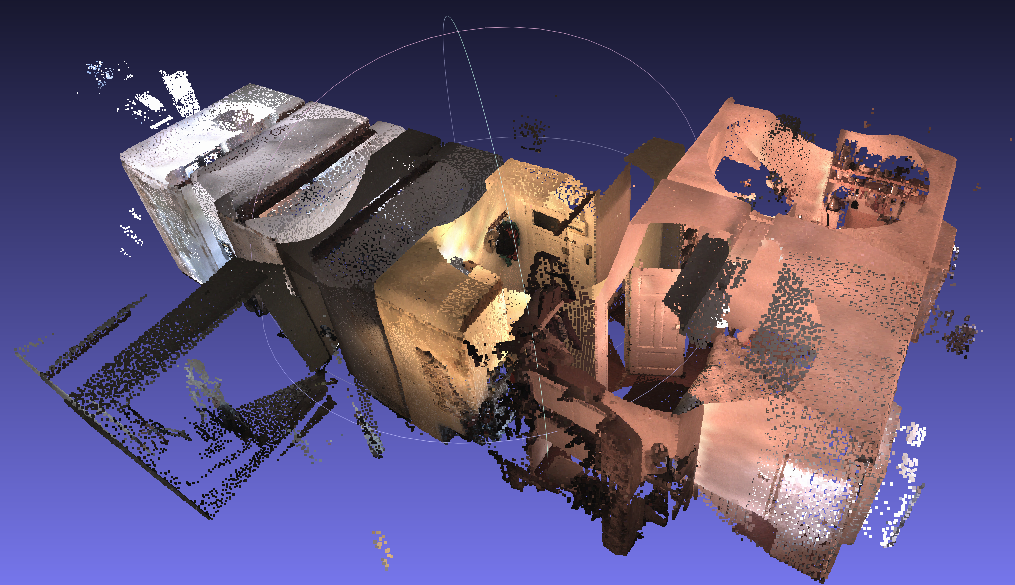
\includegraphics[width=\textwidth]{2014-02-28-101630_1015x585_scrot.png}
\caption{appartement}
\end{figure}
\end{frame}

\begin{frame}{$\beta=10$}
\begin{figure}[hbtp]
\centering
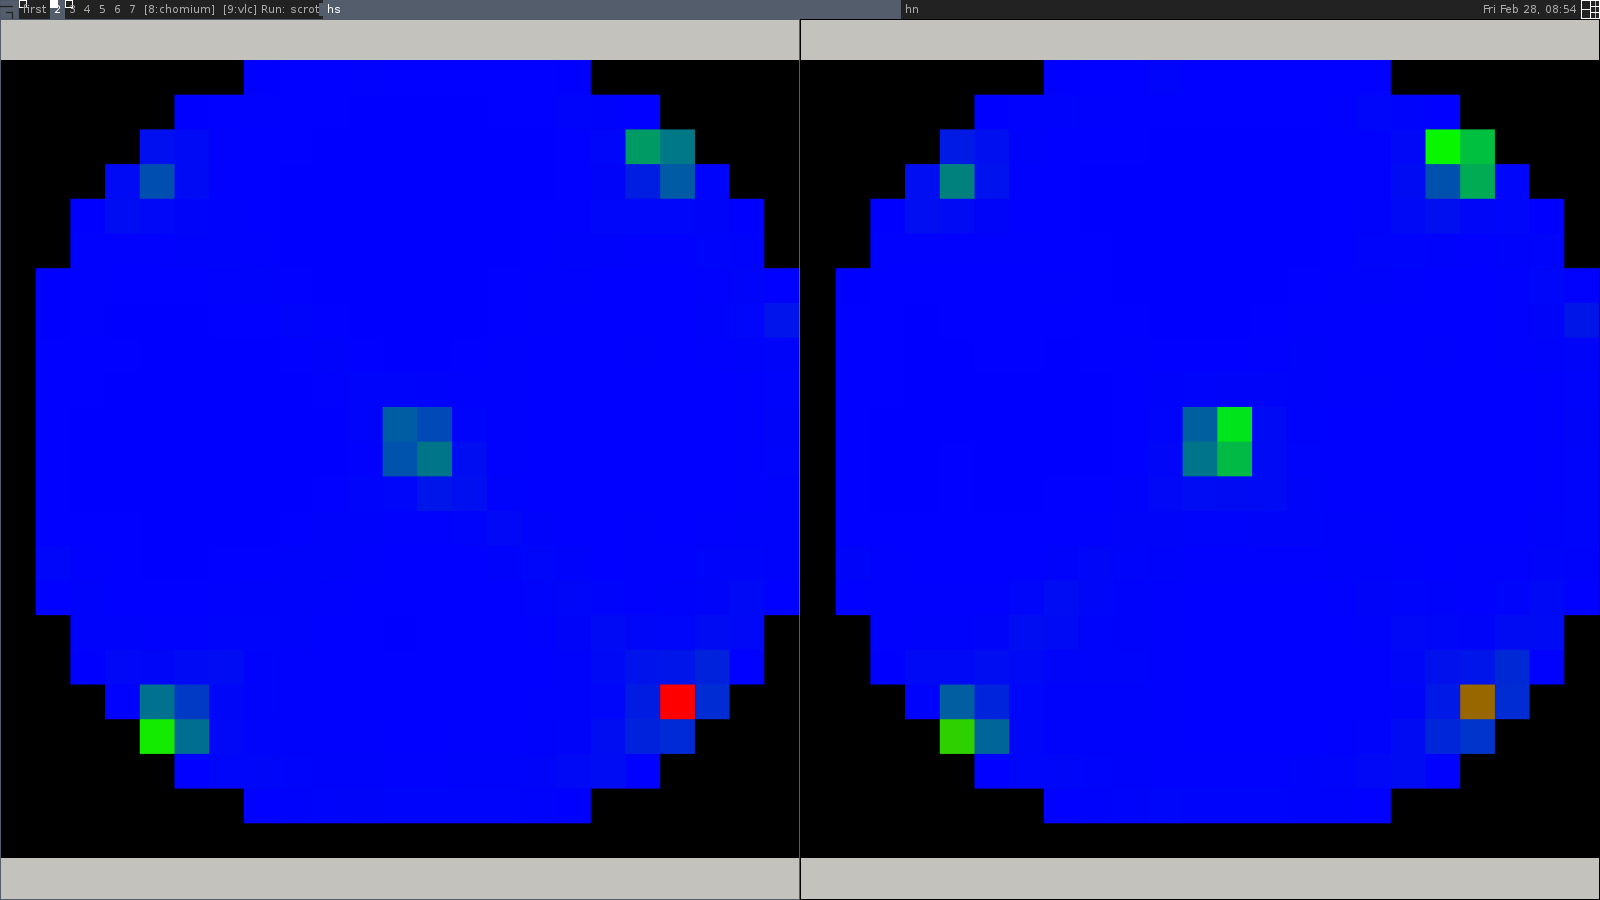
\includegraphics[width=\textwidth]{2014-02-28-085518_1600x900_scrot.png}
\caption{gauss $\beta=10$}
\end{figure}
\end{frame}

\begin{frame}{$\beta=90$}
\begin{figure}[hbtp]
\centering
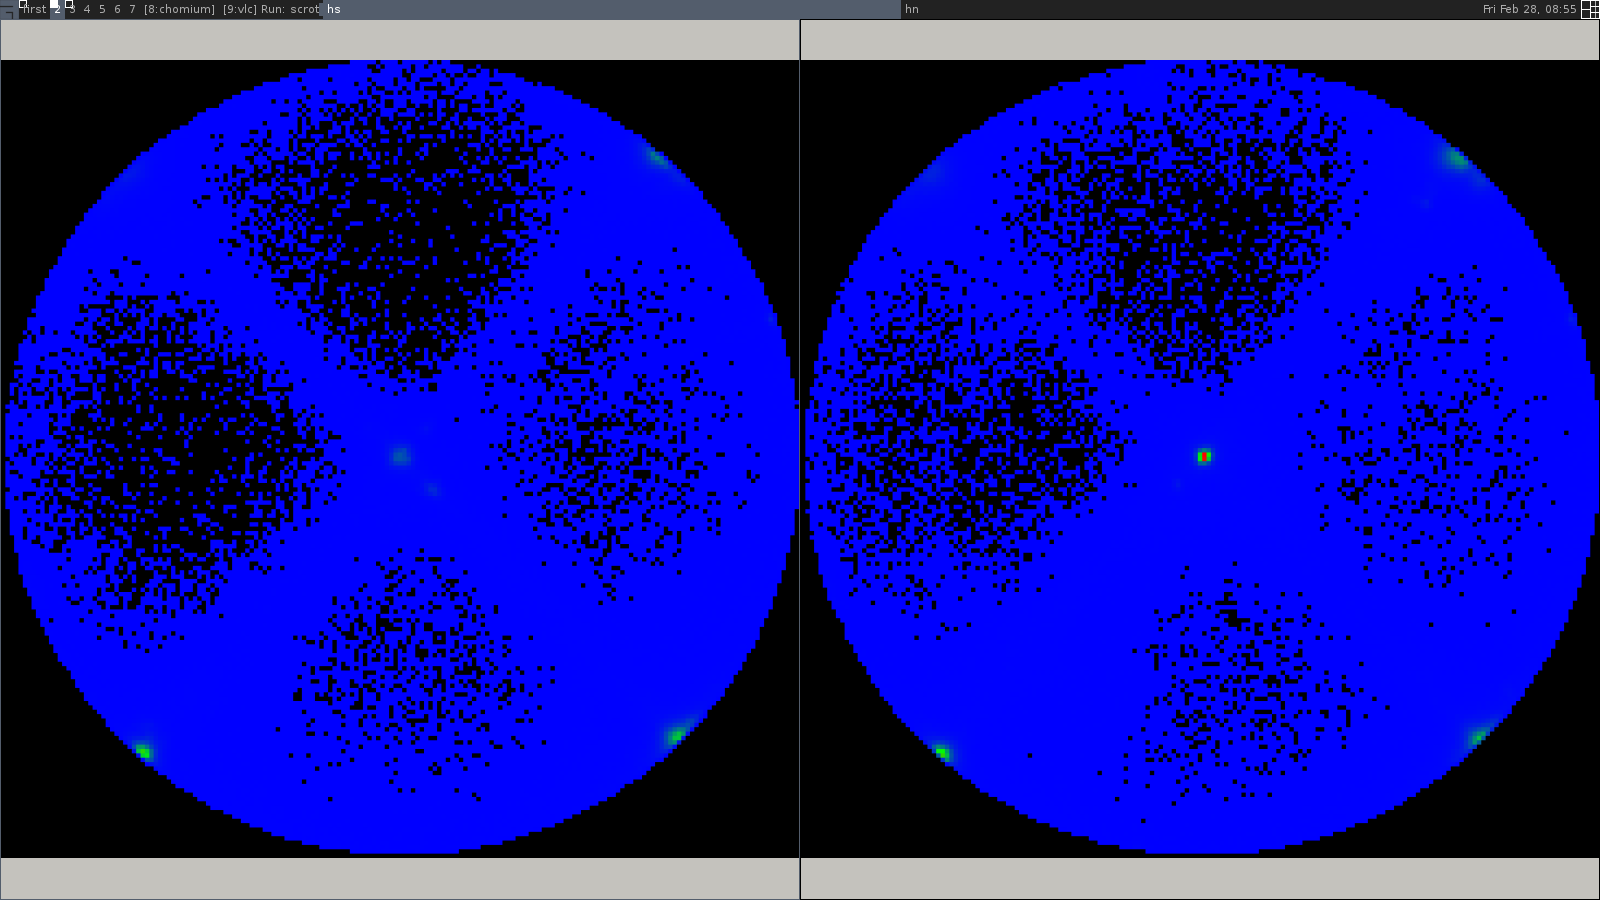
\includegraphics[width=\textwidth]{2014-02-28-085627_1600x900_scrot.png}
\caption{gauss $\beta=90$}
\end{figure}

\end{frame}
\begin{frame}{$\beta=1000$}
\begin{figure}[hbtp]
\centering
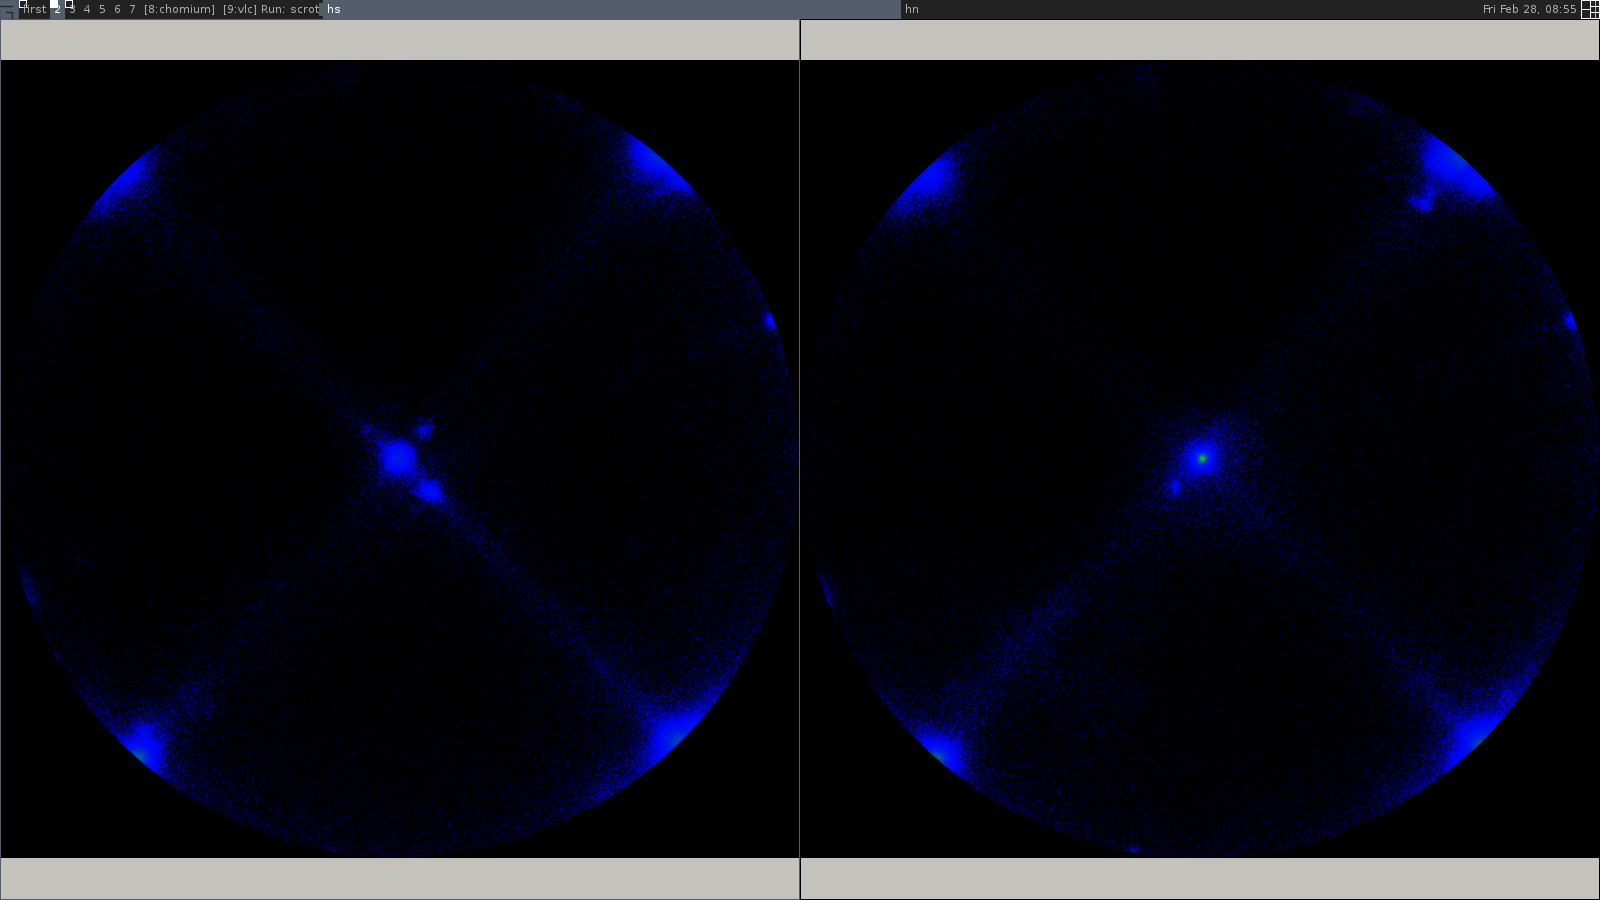
\includegraphics[width=\textwidth]{2014-02-28-085643_1600x900_scrot.png}
\caption{gauss $\beta=1000$}
\end{figure}
\end{frame}


\begin{frame}{église $S^t$ Jean}
\begin{multicols}{2}
\begin{figure}[hbtp]
\centering
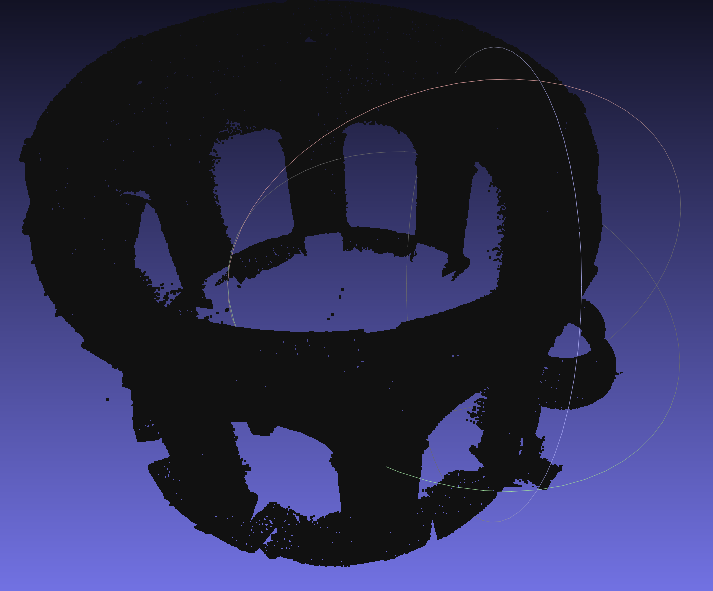
\includegraphics[width=\columnwidth]{2014-02-28-102010_713x591_scrot.png}
\caption{église $S^t$ Jean}
\end{figure}

\columnbreak

\begin{figure}[hbtp]
\centering
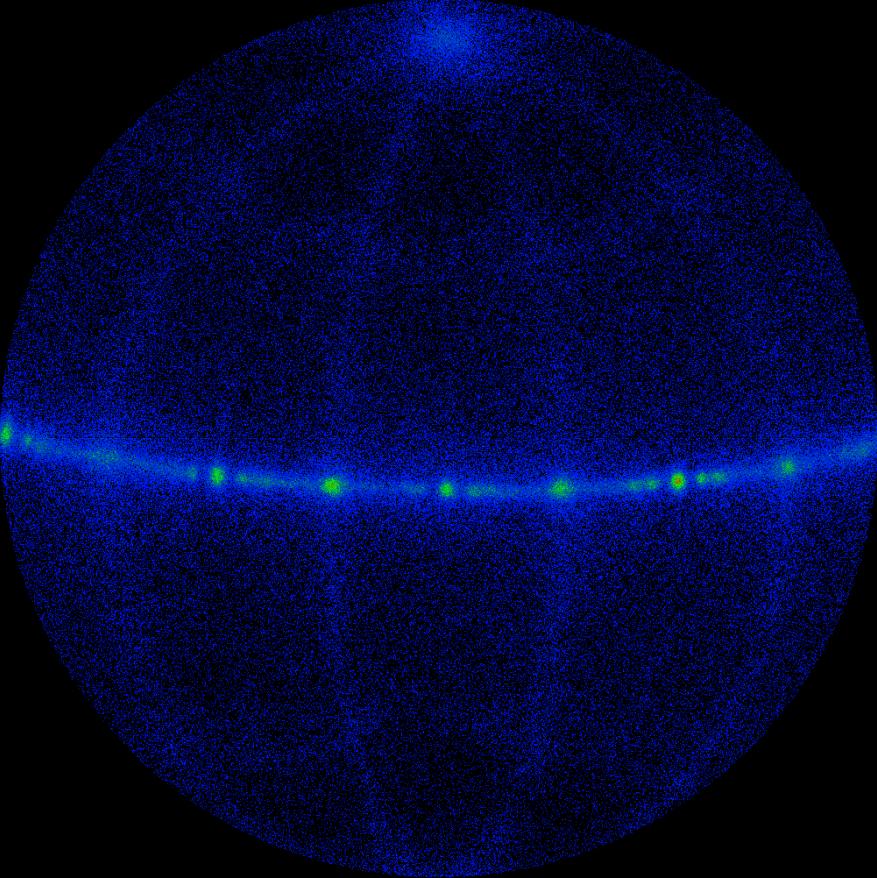
\includegraphics[width=\columnwidth]{gauss_st_jean.png}
\caption{gauss $\beta=1000$}
\end{figure}
\end{multicols}

\end{frame}

\section{Détection de plan}
\begin{frame}{TODO}
detection normal dir
\end{frame}


\begin{frame}{}
\begin{multicols}{2}

\columnbreak

\end{multicols}
\end{frame}


\begin{frame}{Distribution des plans selon la normale}

\begin{figure}[hbtp]
\centering
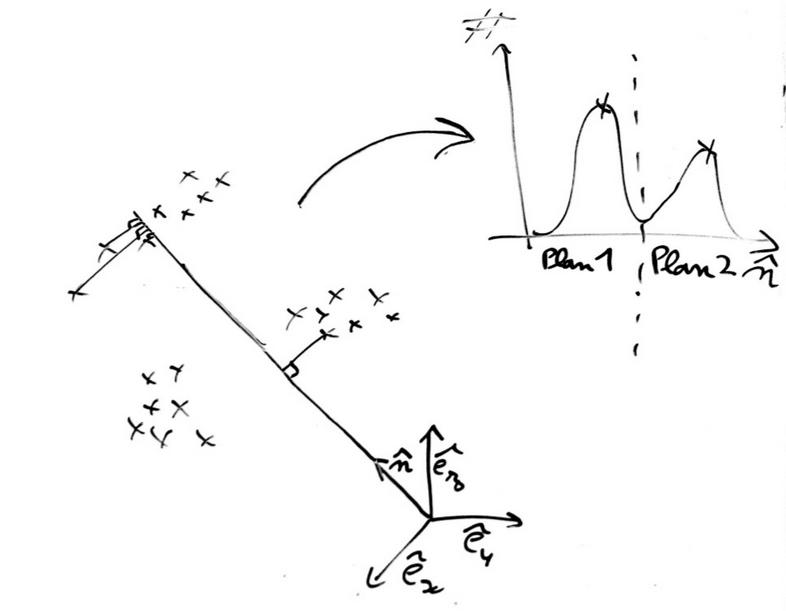
\includegraphics[width=.7\textwidth]{normal_to_hist.png}
\caption{Distribution des plans selon la normale}
\end{figure}
\end{frame}

\begin{frame}{Exemple de distributions}

\begin{figure}[hbtp]
\centering
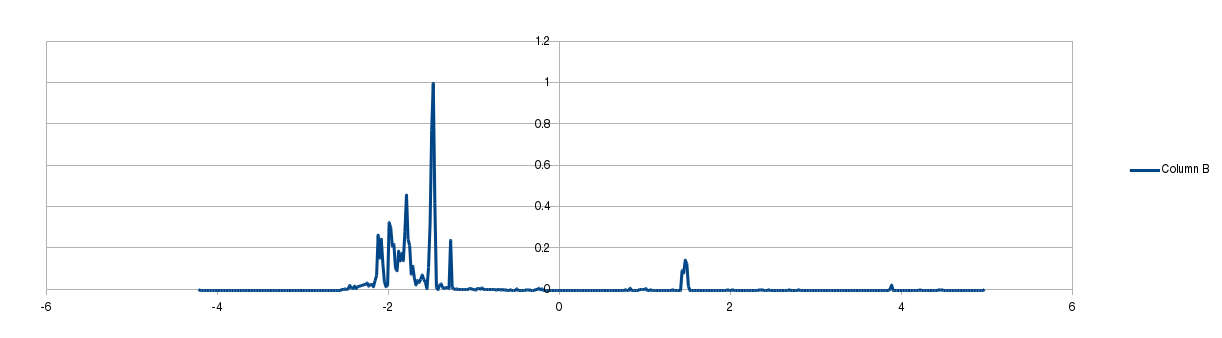
\includegraphics[width=\columnwidth]{distribution_along_normal.png}
\caption{gauss $\beta=1000$}
\end{figure}
\begin{figure}[hbtp]
\centering
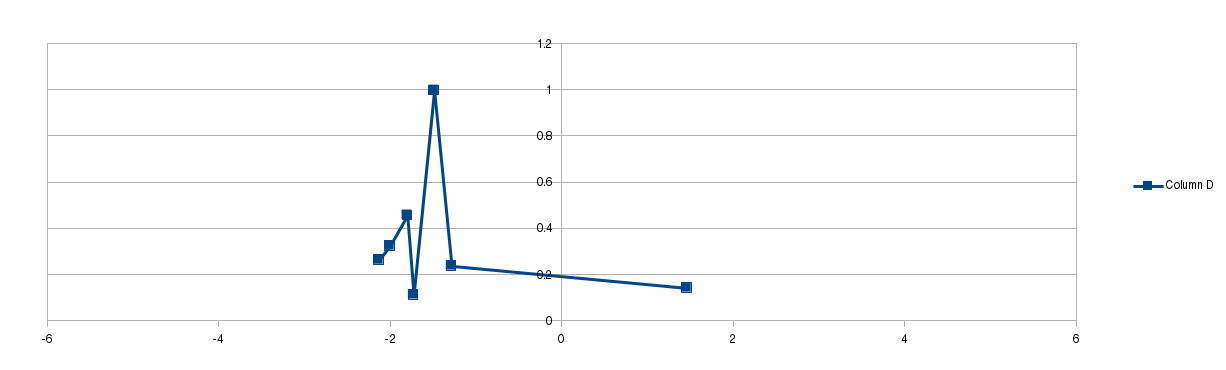
\includegraphics[width=\columnwidth]{distribution_along_normal_max.png}
\caption{gauss $\beta=1000$}
\end{figure}

\end{frame}


\begin{frame}{Exemple de distributions}

\begin{figure}[hbtp]
\centering
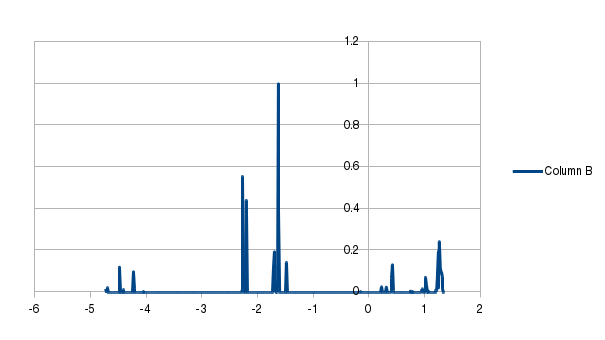
\includegraphics[width=.5\textwidth]{distribution_along_normal1.png}
\end{figure}
\begin{figure}[hbtp]
\centering
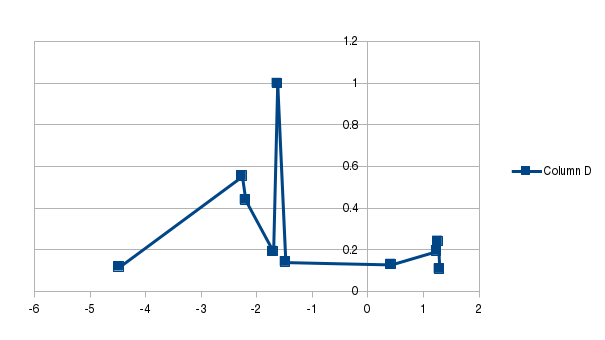
\includegraphics[width=.5\textwidth]{distribution_along_normal_max1.png}
\end{figure}

\end{frame}

\section{Plan}



\begin{frame}{Image de Référence}
\begin{figure}[hbtp]
\centering
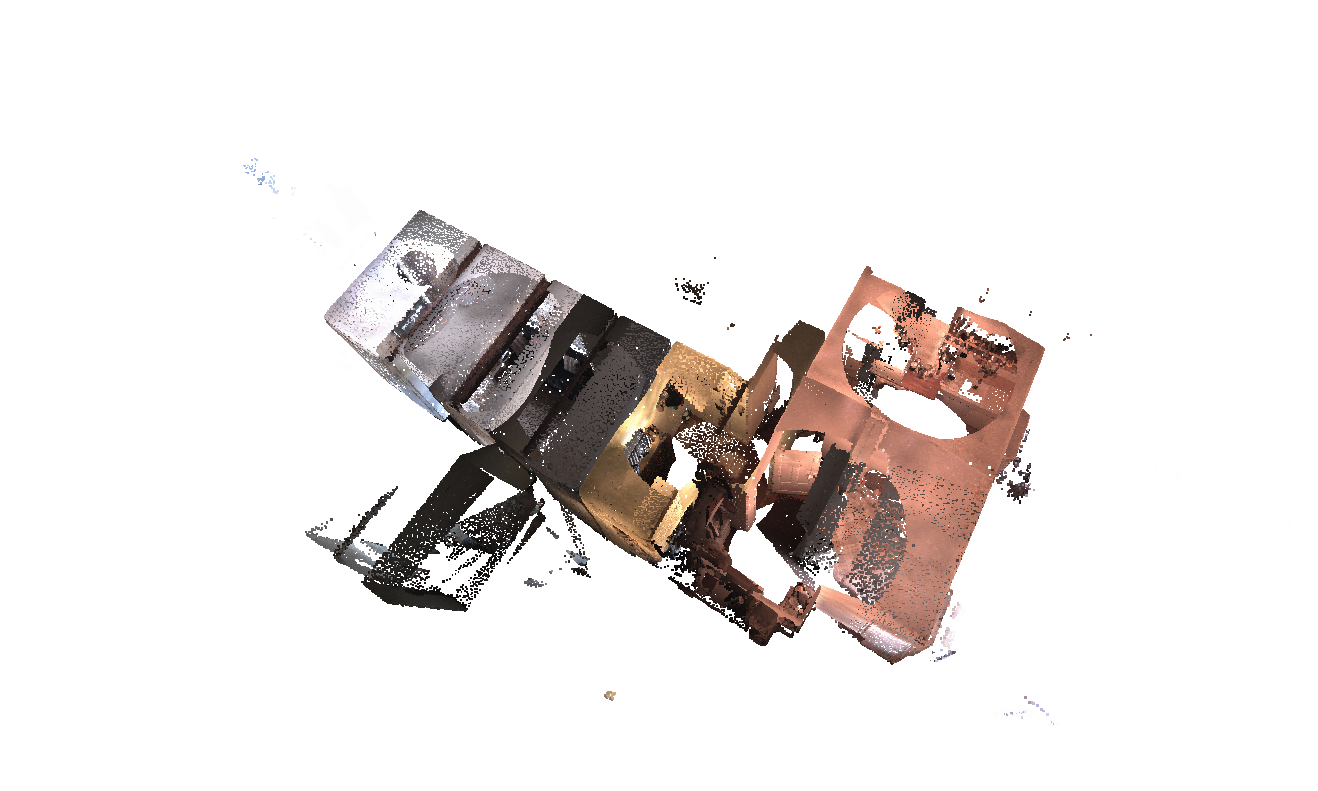
\includegraphics[width=\columnwidth]{appart01.png}
\caption{appartement}
\end{figure}
\end{frame}

\begin{frame}{Plan détectés}
\begin{figure}[hbtp]
\centering
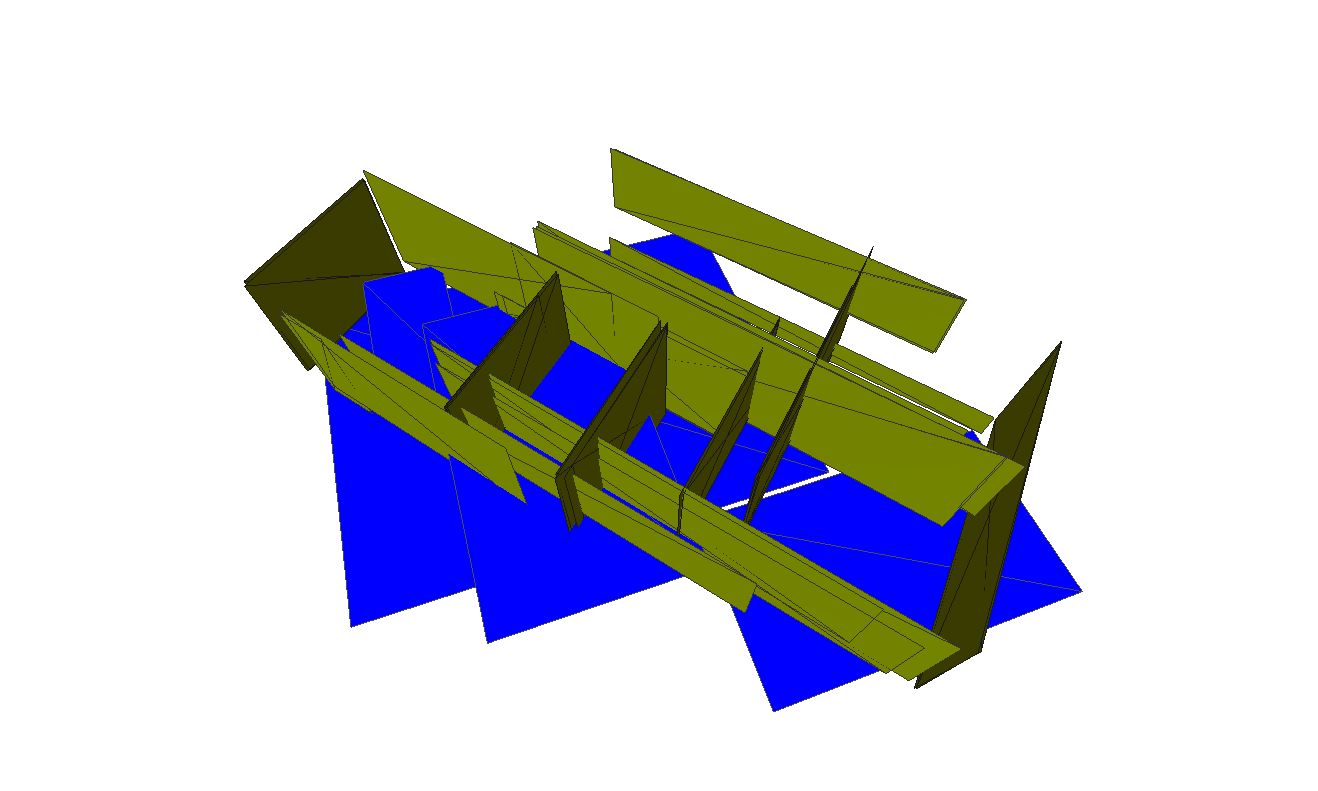
\includegraphics[width=\columnwidth]{appart04.png}
\caption{appartement}
\end{figure}
\end{frame}



\begin{frame}{Comparaison}
\begin{multicols}{2}
\begin{figure}[hbtp]
\centering
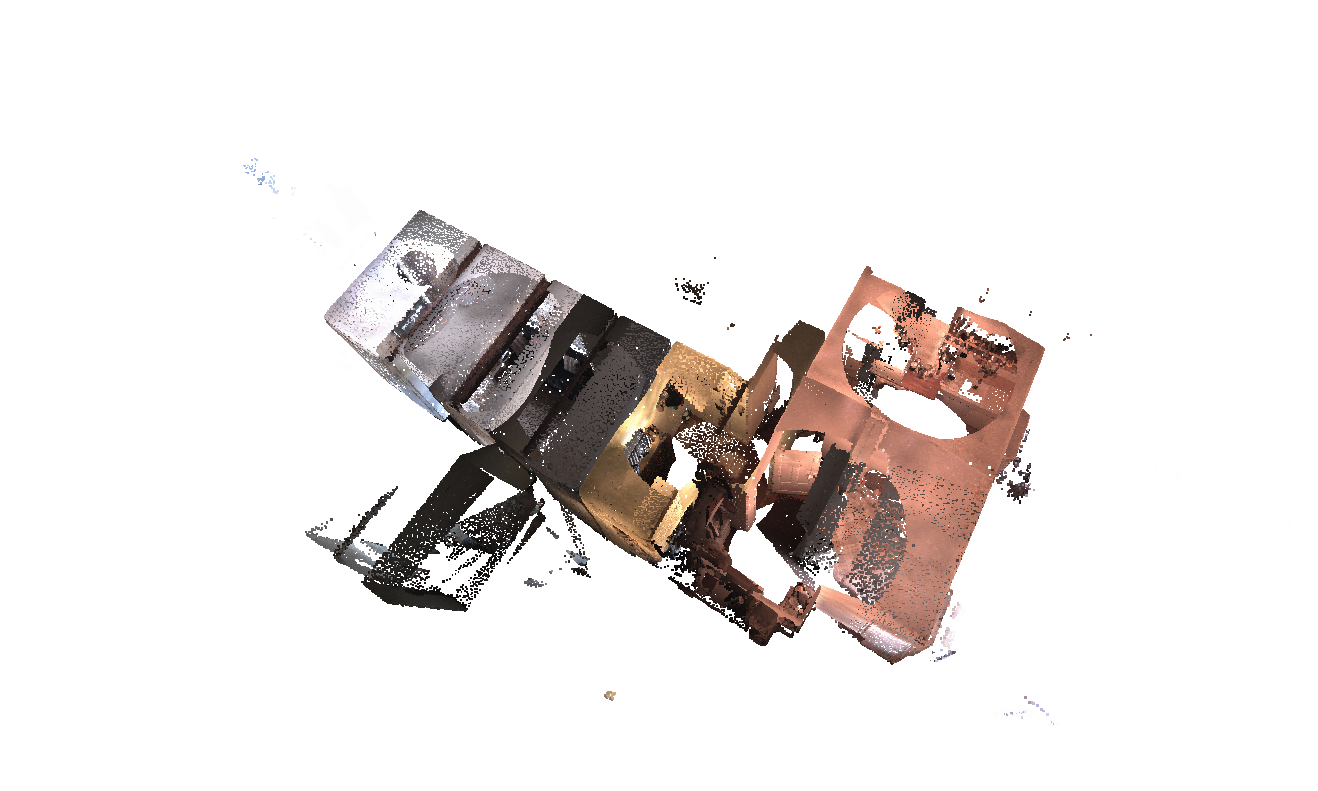
\includegraphics[width=1.3\columnwidth]{appart01.png}
\caption{appartement}
\end{figure}

\columnbreak
\begin{figure}[hbtp]
\centering
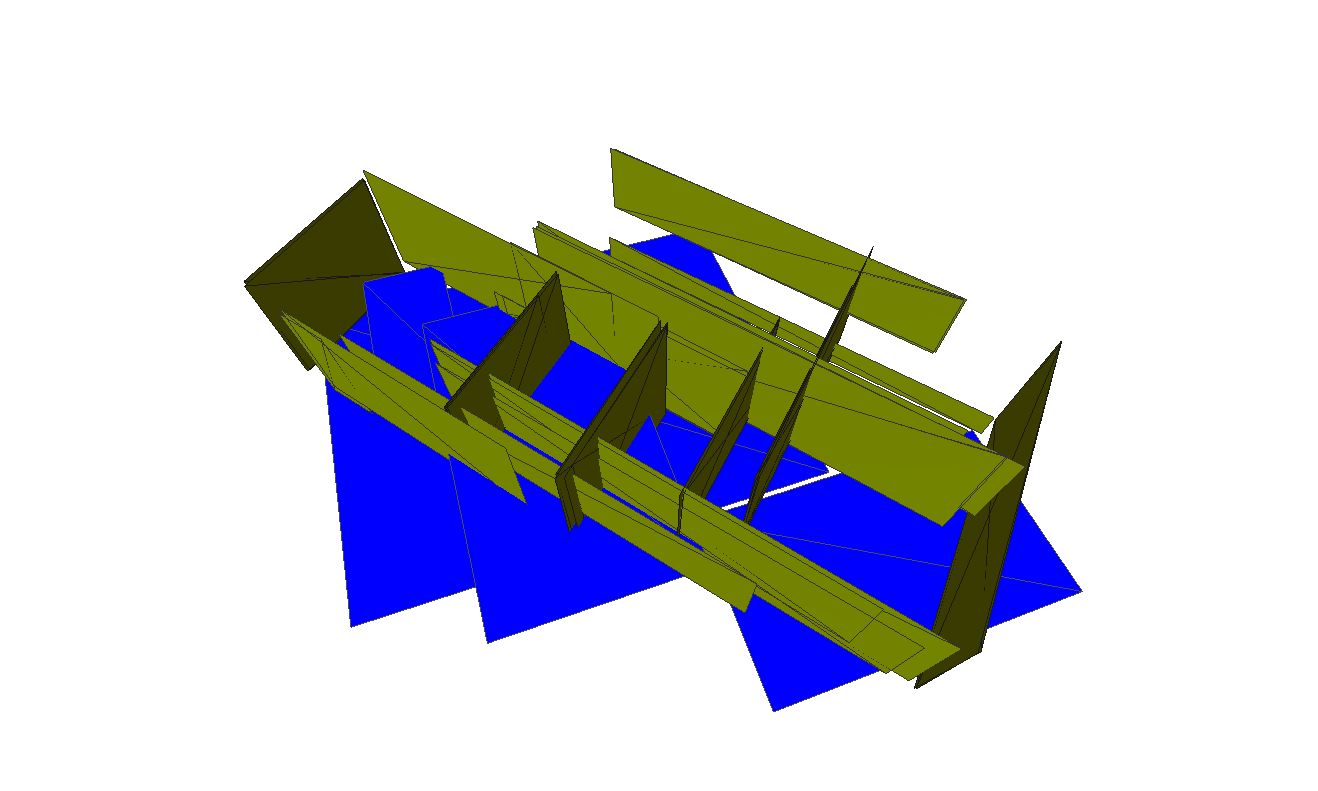
\includegraphics[width=1.3\columnwidth]{appart04.png}
\caption{appartement}
\end{figure}

\end{multicols}
\end{frame}



\begin{frame}{Plan détectés}
\begin{figure}[hbtp]
\centering
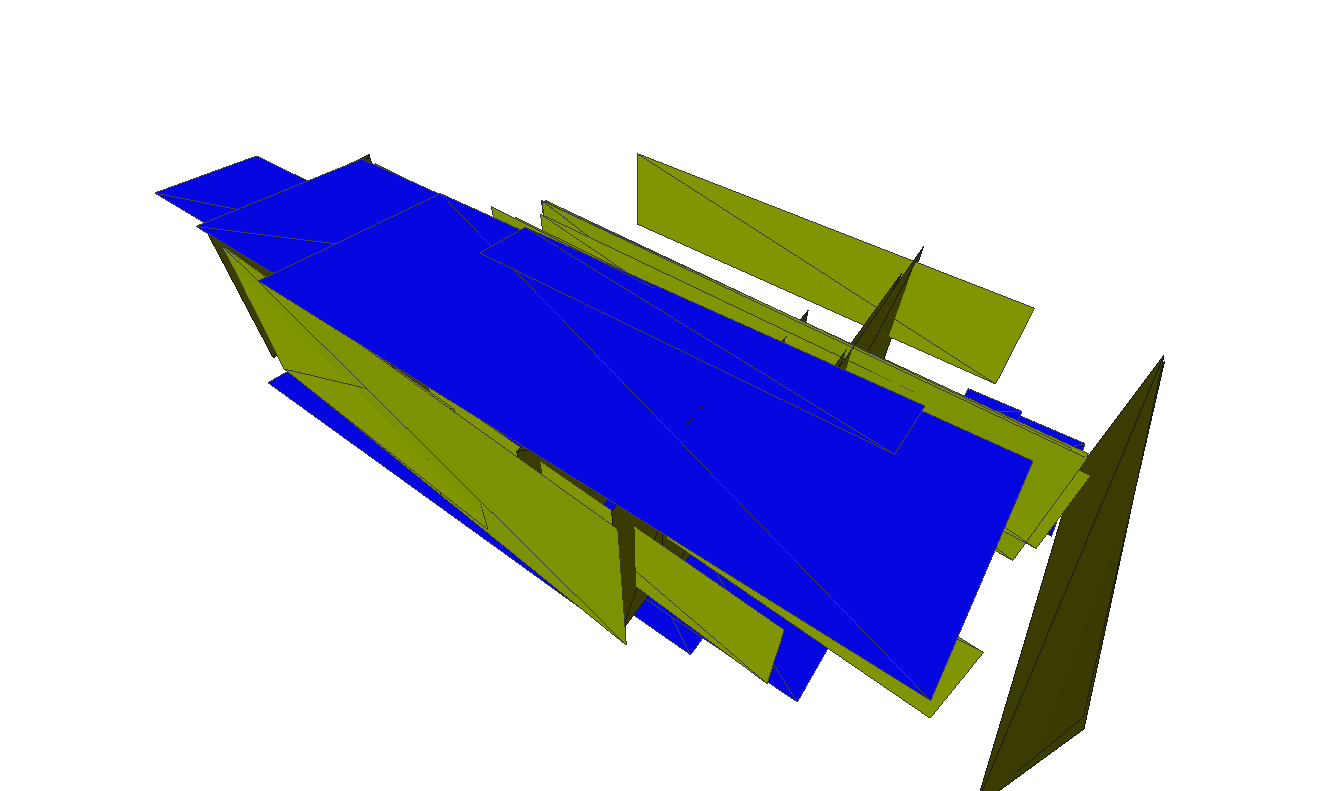
\includegraphics[width=\columnwidth]{appart06.png}
\caption{appartement}
\end{figure}
\end{frame}
\begin{frame}{Plan détectés}
\begin{figure}[hbtp]
\centering
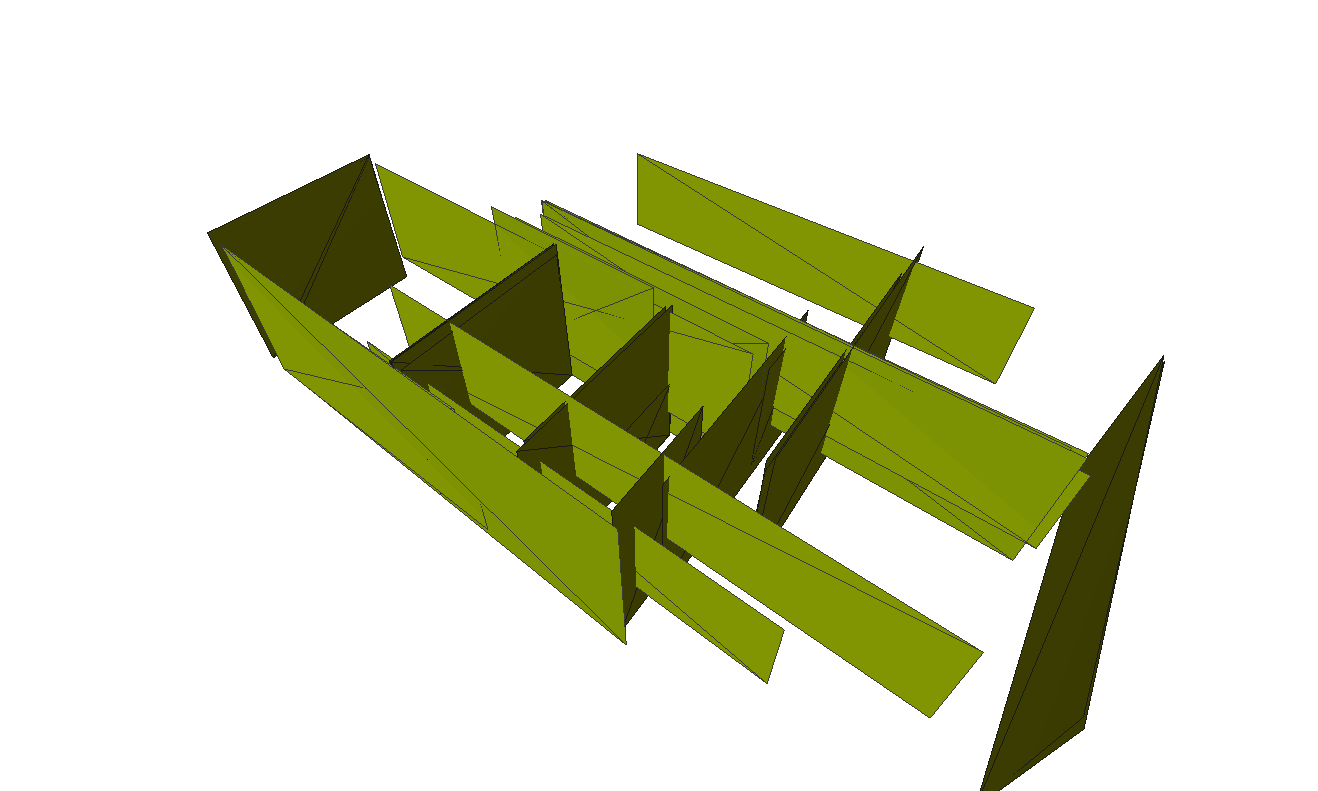
\includegraphics[width=\columnwidth]{appart05.png}
\caption{appartement}
\end{figure}
\end{frame}

\begin{frame}{Plan sans clusteriser les normales}
\begin{figure}[hbtp]
\centering
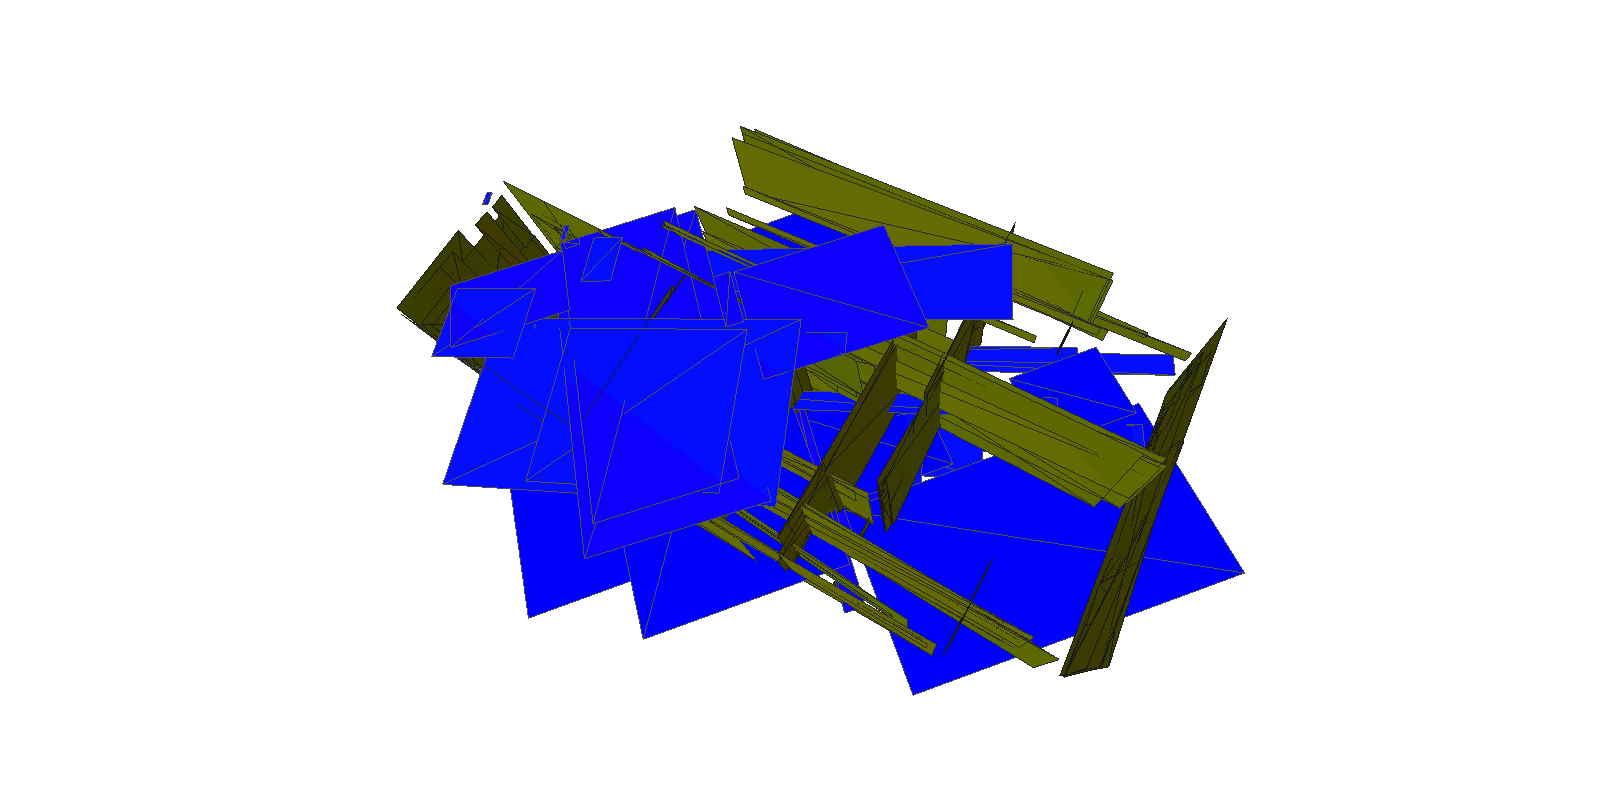
\includegraphics[width=\columnwidth]{appart00.png}
\caption{appartement}
\end{figure}
\end{frame}




\begin{frame}{•}
\end{frame}

\end{document}